% $Header: /cvsroot/latex-beamer/latex-beamer/solutions/conference-talks/conference-ornate-20min.en.tex,v 1.6 2004/10/07 20:53:08 tantau Exp $

\documentclass{beamer}

\mode<presentation>
{
%  \usetheme{Hannover}
\usetheme{Hannover}
% or ...

  %\setbeamercovered{transparent}
  % or whatever (possibly just delete it)
}
% \setbeamercolor{footlinecolor}{fg=black,bg=blue}
%\setbeamertemplate{footline}[frame number]

\setbeamertemplate{footline}
{
  \leavevmode
  \hbox{  \hspace{-1em}\begin{beamercolorbox}[wd=.4\paperwidth,ht=2.25ex,dp=1ex,left]{author
        in head/foot}    \usebeamerfont{subsection in head/foot} %~~~~SEHPCCSE 2016
  \end{beamercolorbox}  \hspace{-1em}
  \begin{beamercolorbox}[wd=.62\paperwidth,ht=2.25ex,dp=1ex,right]{author in head/foot}    \usebeamerfont{author in head/foot}\hspace*{18em}
    \insertframenumber{} / \inserttotalframenumber\hspace*{5ex}
  \end{beamercolorbox}}
  \vskip0pt
}

\usepackage[english]{babel}
% or whatever

\usepackage[latin1]{inputenc}
% or whatever

\usepackage{times}
%\usepackage[T1]{fontenc}
% Or whatever. Note that the encoding and the font should match. If T1
% does not look nice, try deleting the line with the fontenc.
%\usepackage{logictheme}

\usepackage{multirow}
\usepackage{totpages}

\usepackage{booktabs}

\usepackage[round]{natbib}
\usepackage[multiple]{footmisc}

\usepackage{listings}
\usepackage{xcolor}

\lstset{
    language=Python,
    basicstyle=\ttfamily\small,
    numbers=left,
    numberstyle=\tiny,
    frame=single,
    breaklines=true,
    showstringspaces=false
}

\usepackage{hyperref}
\hypersetup{colorlinks=true,
    linkcolor=blue,
    citecolor=blue,
    filecolor=blue,
    urlcolor=blue,
    unicode=false}
\urlstyle{same}

\usepackage{pifont}
\usepackage{amsmath,amsfonts,xspace,xcolor,url}
\newcommand{\cross}{\ding{55}}

\renewcommand{\arraystretch}{1.1} %so that tables with equations do not look crowded

\pgfdeclareimage[height=0.7cm]{logo}{McMasterLogo}
\title[\pgfuseimage{logo}] % (optional, use only with long paper titles)
{RSE-Supported Scientific Software Standardization}

%\subtitle
%{Include Only If Paper Has a Subtitle}

%\author[Slide \thepage~of \pageref{TotPages}] % (optional, use only with lots of
                                              % authors)
\author[Smith et al.]
{Spencer Smith, Christian Brodbeck, Zhangwenchi Li}
% - Give the names in the same order as the appear in the paper.
% - Use the \inst{?} command only if the authors have different
%   affiliation.

\institute[McMaster University] % (optional, but mostly needed)
{
  Computing and Software Department\\
  Faculty of Engineering\\
  McMaster University\\
  Hamilton, Ontario, Canada\\
}
% - Use the \inst command only if there are several affiliations.
% - Keep it simple, no one is interested in your street address.

\date[Sept 8, 2026] % (optional, should be abbreviation of conference name)
{IRSC26, Sept 8, 2026}
% - Either use conference name or its abbreviation.
% - Not really informative to the audience, more for people (including
%   yourself) who are reading the slides online

\subject{computational science and engineering, software engineering,
verification and validation, verification and validation plan, assurance case}
% This is only inserted into the PDF information catalog. Can be left
% out. 

% If you have a file called "university-logo-filename.xxx", where xxx
% is a graphic format that can be processed by latex or pdflatex,
% resp., then you can add a logo as follows:

%\pgfdeclareimage[height=0.5cm]{Mac-logo}{McMasterLogo}
%\logo{\pgfuseimage{Mac-logo}}

% Delete this, if you do not want the table of contents to pop up at
% the beginning of each subsection:
% \AtBeginSubsection[]
% {
%   \begin{frame}<beamer>
%     \frametitle{Outline}
%     \tableofcontents[currentsection,currentsubsection]
%   \end{frame}
% }

% If you wish to uncover everything in a step-wise fashion, uncomment
% the following command: 

%\beamerdefaultoverlayspecification{<+->}

\beamertemplatenavigationsymbolsempty 

\begin{document}

%%%%%%%%%%%%%%%%%%%%%%%%%%%%%%%%%%%%%%
\hoffset=-.4in %removing side bar for these frames
\begin{frame}[plain]

\titlepage

% different flavour talk - software engineering technique applied to RS
% survey attendees - who does VnV? who plans VnV at start of project?

\end{frame}
\hoffset=0in %restore
%%%%%%%%%%%%%%%%%%%%%%%%%%%%%%%%%%%%%%

\section[Abstract]{Abstract}

%%%%%%%%%%%%%%%%%%%%%%%%%%%%%%%%%%%%%%

\begin{frame}

\frametitle{Abstract}

\begin{itemize}

\item Technical debt $\rightarrow$ Standardization $\rightarrow$ Interface
\item Steps
\begin{enumerate}
\item Should you standardize?
\item Backward compatibility?
\item Learn necessary domain knowledge
\item Document current design architecture
\item Abstraction to isolate interface
\item Implementation
\item Verification
\item Migration plan
\end{enumerate}
\item Guidelines
\begin{itemize}
  \item Question-driven learning
  \item Information hiding  
  \item Task decomposition
  \item Multi-layered testing 
  \item Deprecation warnings
\end{itemize}
\item Case study: Eelbrain-BIDS

\end{itemize}

\end{frame}

%%%%%%%%%%%%%%%%%%%%%%%%%%%%%%%%%%%%%%

\section[Background]{Background}

%%%%%%%%%%%%%%%%%%%%%%%%%%%%%%%%%%%%%%

\begin{frame}

\frametitle{Eelbrain-BIDS}


\begin{itemize}
\item Magnetoencephalography (MEG) 
\item Electroencephalography (EEG) 
\item Stimulus, then record a multi-channel time series
\end{itemize}

\centering
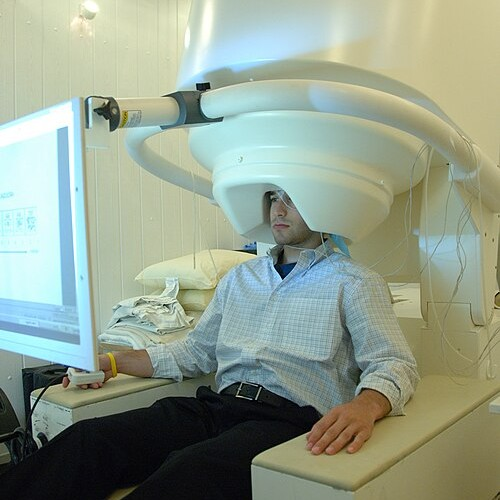
\includegraphics[width=0.35\textwidth]{../Resources/meg_device.jpg}
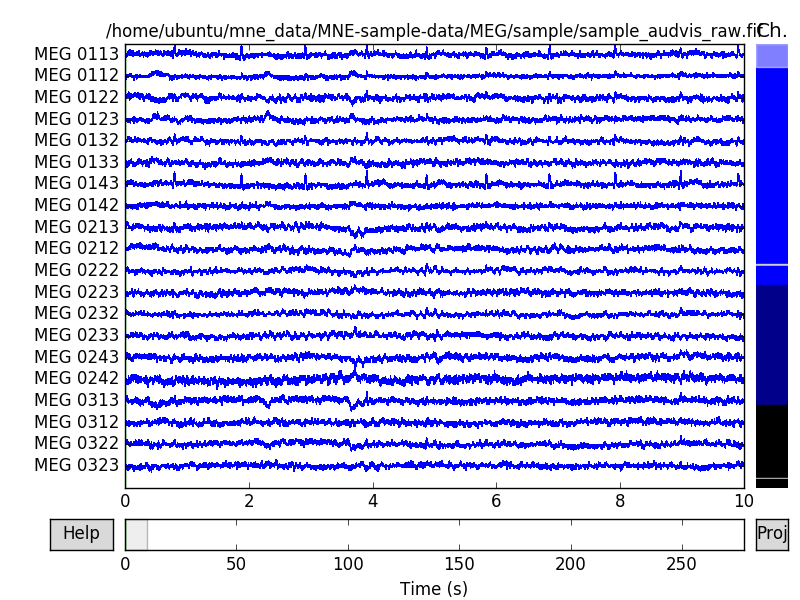
\includegraphics[width=0.5\textwidth]{../Resources/meg_data.png}\\[0.4em]{\footnotesize MEG device and the recorded multi-channel data}


\end{frame}

%%%%%%%%%%%%%%%%%%%%%%%%%%%%%%%%%%%%%%

\begin{frame}[fragile]

\frametitle{Eelbrain-BIDS}


\begin{itemize}

\item Open-source Python library for M/EEG data analysis\footnote{\href{https://github.com/Eelbrain/Eelbrain}{https://github.com/Eelbrain/Eelbrain}}
\item BIDS (Brain Imaging Data Structure) is a community standard for organizing and sharing brain data
\item The Eelbrain-BIDS project upgraded the input dataset format of Eelbrain from a custom format to BIDS

\end{itemize}

\centering
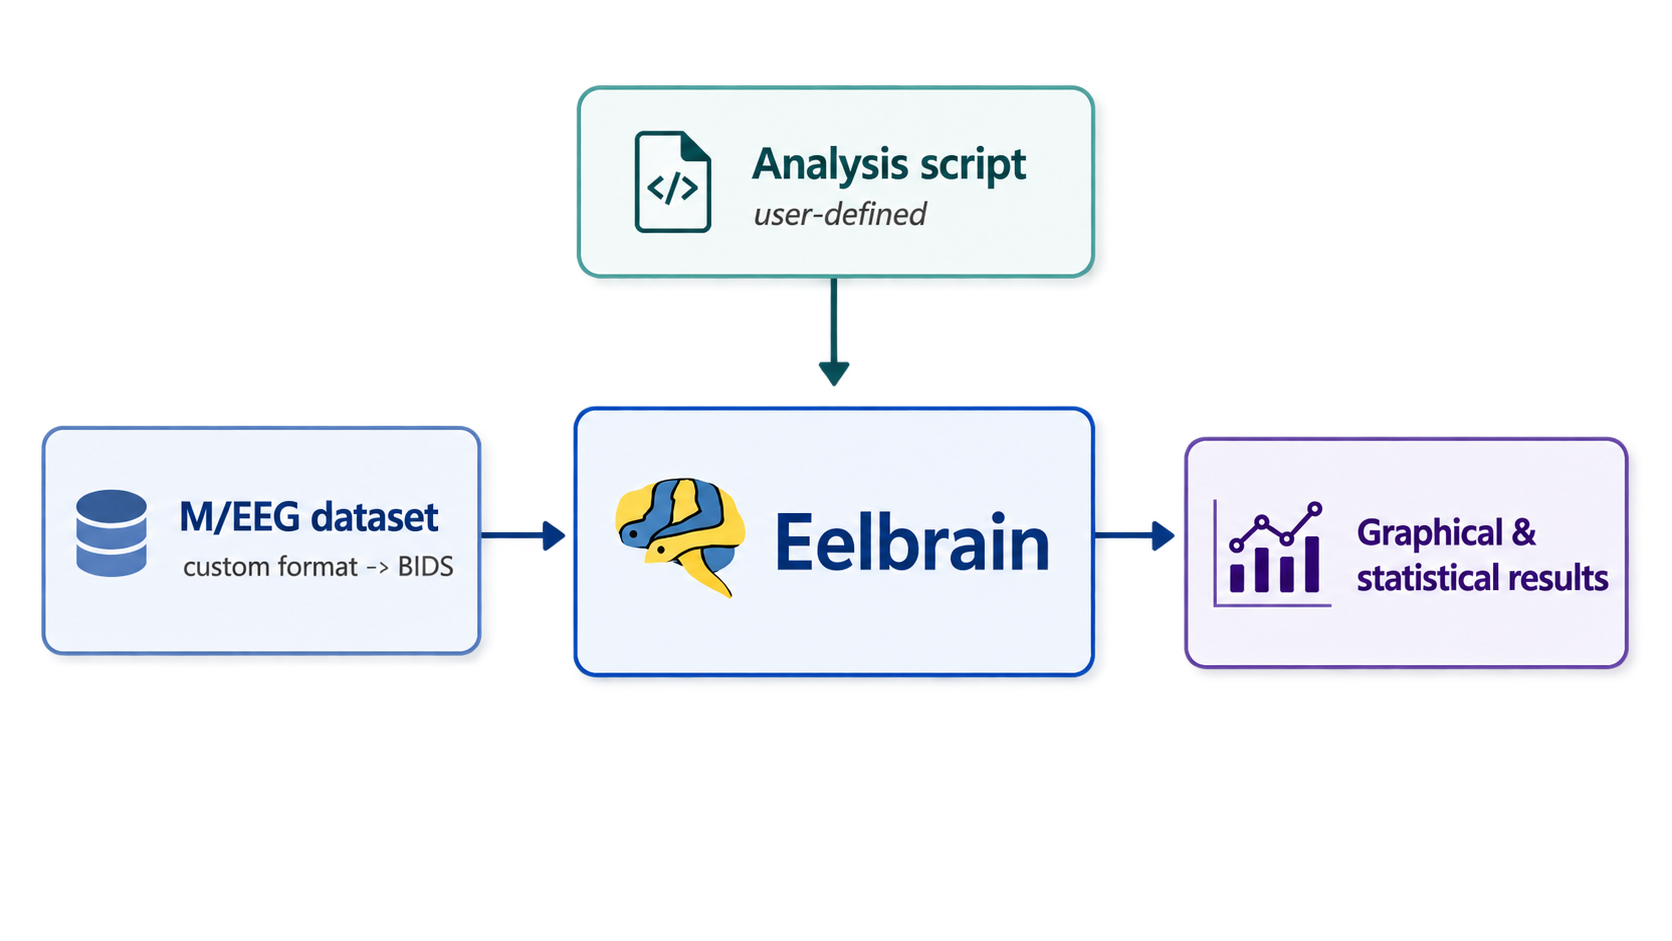
\includegraphics[width=0.8\textwidth]{../Resources/relationship.png}


\end{frame}

%%%%%%%%%%%%%%%%%%%%%%%%%%%%%%%%%%%%%%

\begin{frame}

\frametitle{Technical Debt and Standardization}

Technical debt\footnote{Term first used by \citet{Ward1992}} $\rightarrow$ Standardization $\rightarrow$ Interface standards

\centering
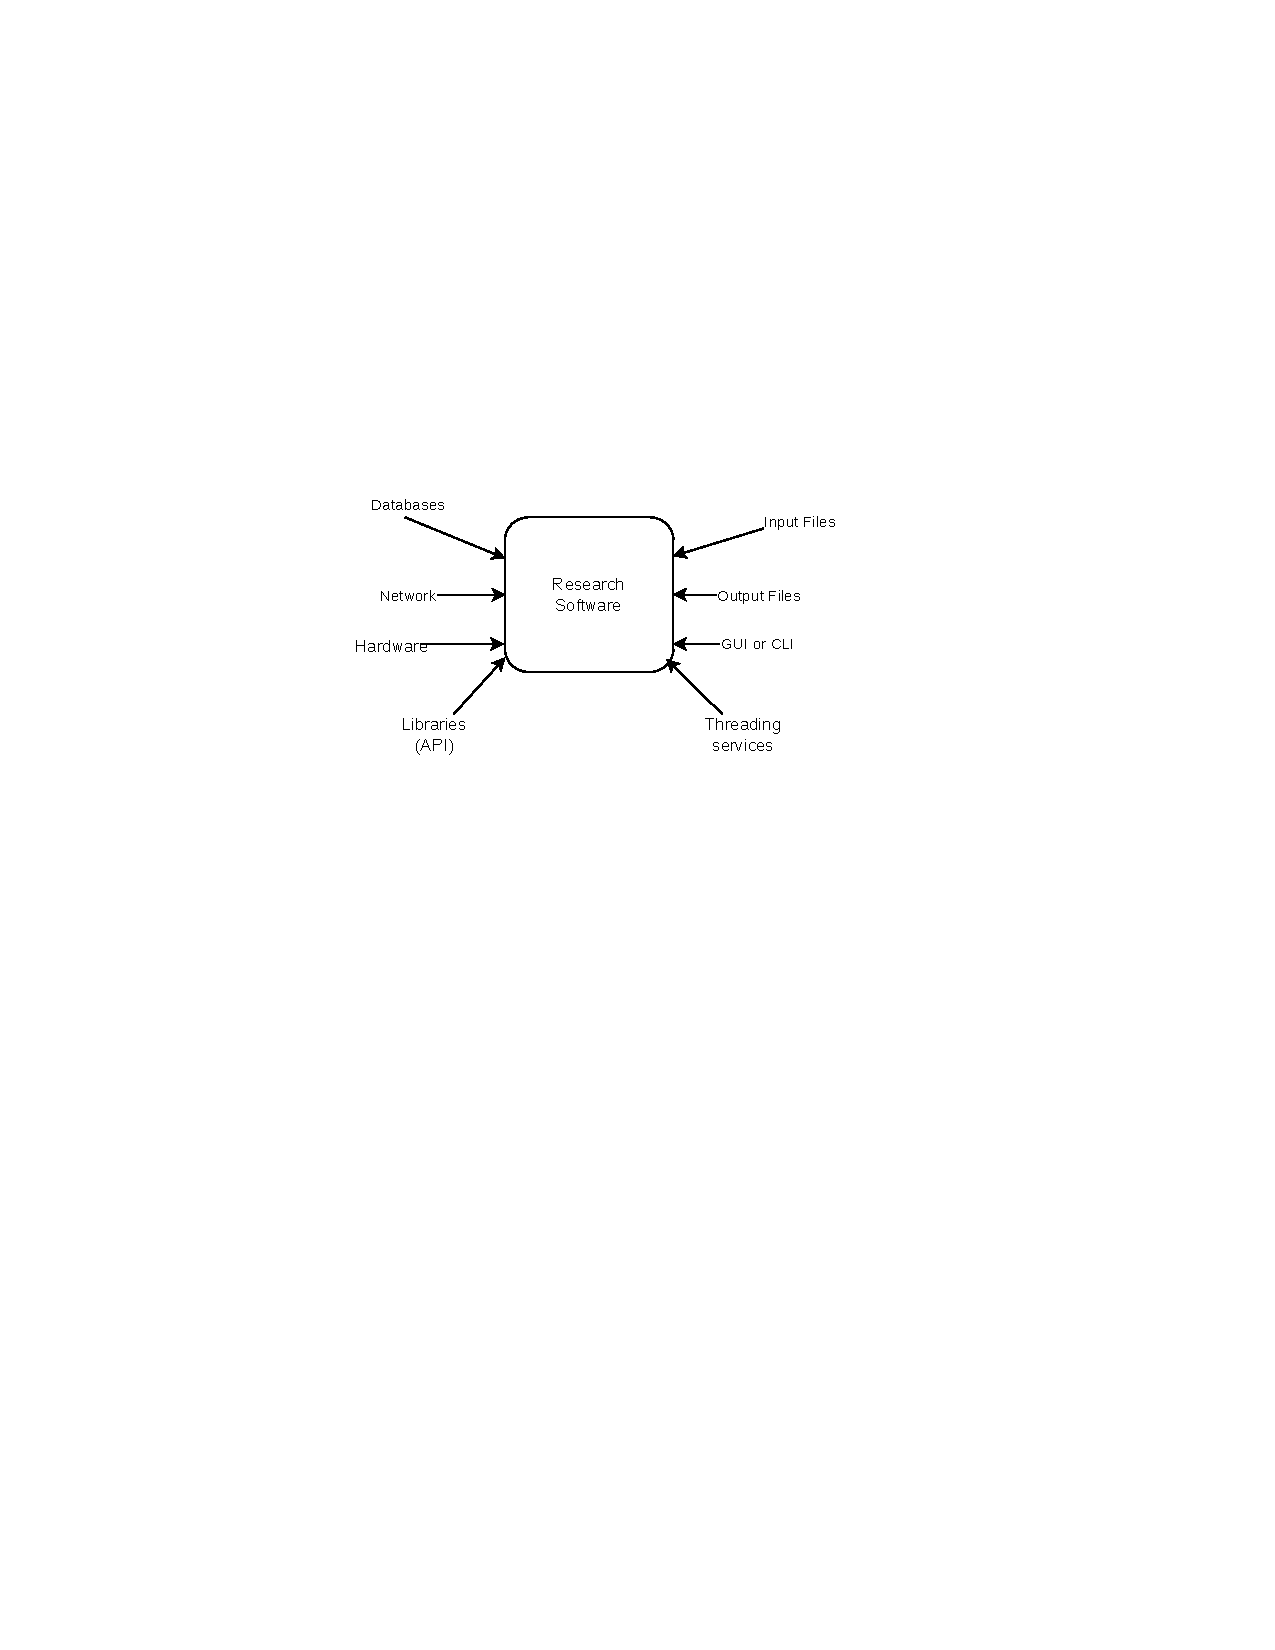
\includegraphics[width=0.8\textwidth]{../Resources/StdInt.pdf}

%technical debt: the cost of additional rework caused by choosing an easy solution now instead of using a better approach that would take longer
%standardization: a set of community agreed-upon rules, guidelines, or characteristics for a particular activity or field
%neglect of standardization is a special kind of technical debt - related to interfaces
%scope - looking at standard interface and standard data format, not standard algorithms or standard software architecture, or standard methodology etc.
%internals are NOT standardized, but the interface is standardized
\end{frame}

%%%%%%%%%%%%%%%%%%%%%%%%%%%%%%%%%%%%%%

\section[Steps]{Idealized Steps}

%%%%%%%%%%%%%%%%%%%%%%%%%%%%%%%%%%%%%%

\subsection[Standardize?]{Standardize?}

%%%%%%%%%%%%%%%%%%%%%%%%%%%%%%%%%%%%%%
\begin{frame}

\frametitle{Decide Whether to Standardize Interface}

\begin{table}[ht]
\centering
\begin{tabular}{p{0.25\textwidth} p{0.65\textwidth}}
\toprule
\textbf{Pros} & \textbf{Cons} \\
\midrule
Interoperability\footnote{\citet{BasuEtAl2019}}\footnote{\citet{DavidAndGreenstein1990}} % diff tools work together, data sharing
 & Cost of paying technical debt \\ %changing to the new standard will take time+effort
Reproduciblity\footnotemark[3] %facilitates others to reproduce results
 & Have to update to avoid obsolescence \\ %standards evolve, so need to keep up with changes
Reusability\footnotemark[3] %reuse saves time and effort
 & Lose ``benefits'' of closed data formats \\ %proprietary allows to keep control 
Productivity % once people learn, they save time by not having to learn new formats
 & Standard may not be a perfect fit\\ %may be more general than needed
Communication %language for discussion facilitates collaboration
 & Standards may not always be best\\ % a competing technology may be better VHS vs Beta, BlueRay, etc.
\bottomrule
\end{tabular}
\end{table}

\begin{itemize}
\item For Eelbrain moving to BIDS
\begin{itemize}
\item Data sharing since open data is often in BIDS format
\item Community has converged on BIDS
\item Start with six BIDS entities, then add more as needed %full standard is more than needed
\end{itemize}
\end{itemize}
\end{frame}

%%%%%%%%%%%%%%%%%%%%%%%%%%%%%%%%%%%%%%

\subsection[Backward?]{Backward Compatible?}

%%%%%%%%%%%%%%%%%%%%%%%%%%%%%%%%%%%%%%

\begin{frame}

\frametitle{Backward Compatible?}

% famous example of Python 2 to 3
Make Backward Compatible:

\begin{table}[ht]
\centering
\begin{tabular}{p{0.45\textwidth} p{0.45\textwidth}}
\toprule
\textbf{Reasons to keep} & \textbf{Reasons to break} \\
\midrule
Existing code still works & Time+effort to keep\\
Facilitates transition & Future maintenance easier\\ 
Reproducibility & Still have tech.\ debt.\\ 
Protects downstream soft. & Removes constraints\\
User trust & Reduces testing burden\\
\bottomrule
\end{tabular}
\end{table}

\begin{itemize}
\item Depends on current architecture
%\item Info hiding plus strategy pattern %more about behaviour
\item For Eelbrain-BIDS, backward compatibility was dropped -- BIDS makes
different assumptions, too much repetition of code, not enough demand to justify
% BIDS doesn’t assume that the entities are the same between different subjects,
% while the existing system doe
\end{itemize}

\end{frame}

%%%%%%%%%%%%%%%%%%%%%%%%%%%%%%%%%%%%%%

\subsection[Learn]{Learn Necessary Domain Knowledge}

%%%%%%%%%%%%%%%%%%%%%%%%%%%%%%%%%%%%%%

\begin{frame}

\frametitle{Question Driven Learning}

\begin{itemize}
  \item Don't need to understand everything, just enough to understand the interface
  \item Ask domain expert questions\footnote{\citet{DuAndSmith2025-paper}}
  \begin{itemize}
    \item What keyword should I search for?
    \item What is the problem that the software is trying to solve?
    \item What is the context in which the software is used?
    \item What are the typical use cases for the software?
    \item \textbf{What is the approximate scale of the problem.}
    \item What should the user provide as \textbf{inputs}?
    \item What \textbf{output} does the user expect?
    \item What are trends in the output as the input varies?
  \end{itemize}
  \item For a well-documented project, an AI chat-bot could substitute for a domain expert
\end{itemize}

\end{frame}

%%%%%%%%%%%%%%%%%%%%%%%%%%%%%%%%%%%%%%

\subsection[Curr.\ Architec.?]{Current Design Architecture}

%%%%%%%%%%%%%%%%%%%%%%%%%%%%%%%%%%%%%%

\begin{frame}

\frametitle{Document Current Design Architecture}

\begin{itemize}

\item Need current architecture for planning
\item If the interface is well-defined, change can be isolated
\item If not, the first step is to refactor
\item Use information hiding principle\footnote{\citet{parnas_1972}}

\end{itemize}

\end{frame}

%%%%%%%%%%%%%%%%%%%%%%%%%%%%%%%%%%%%%%

\subsection[Abstraction]{Abstraction to Isolate Interface}

%%%%%%%%%%%%%%%%%%%%%%%%%%%%%%%%%%%%%%

\begin{frame}[fragile]

\frametitle{Example ODE Solver}

Solve $\frac{dT_W}{dt} = \frac{1}{\tau_W} (T_C - T_W(t)), T_W(0) = T_\text{init}$

\begin{lstlisting}
    t = [0.0]
    T_W = [T_init]

    while t[-1] < t_end:
        T = T_W[-1]

        # Euler update
        T_new = T + dt * (T_C - T) / tau_W
        t_new = t[-1] + dt

        t.append(t_new)

        T_W.append(T_new)
\end{lstlisting}

\end{frame}

%%%%%%%%%%%%%%%%%%%%%%%%%%%%%%%%%%%%%%

\begin{frame}[fragile]

\frametitle{Abstract Out ODE Solver}

\begin{lstlisting}
def dT_W_dt(t, T_W, T_C, tau_W):
    return (T_C - T_W) / tau_W

# Bind the parameters of our particular ODE
def derivative(t, T_W):
    return dT_W_dt(t, T_W, T_C, tau_W)

t_eval = np.arange(0, t_end + dt, dt)

solution = solve_ivp(
    derivative,
    (0, t_end),
    [T_init],
    t_eval=t_eval,
    method="RK45"
)
\end{lstlisting}

\end{frame}

%%%%%%%%%%%%%%%%%%%%%%%%%%%%%%%%%%%%%%

\begin{frame}

%\frametitle{Current Design Architecture}

\centering
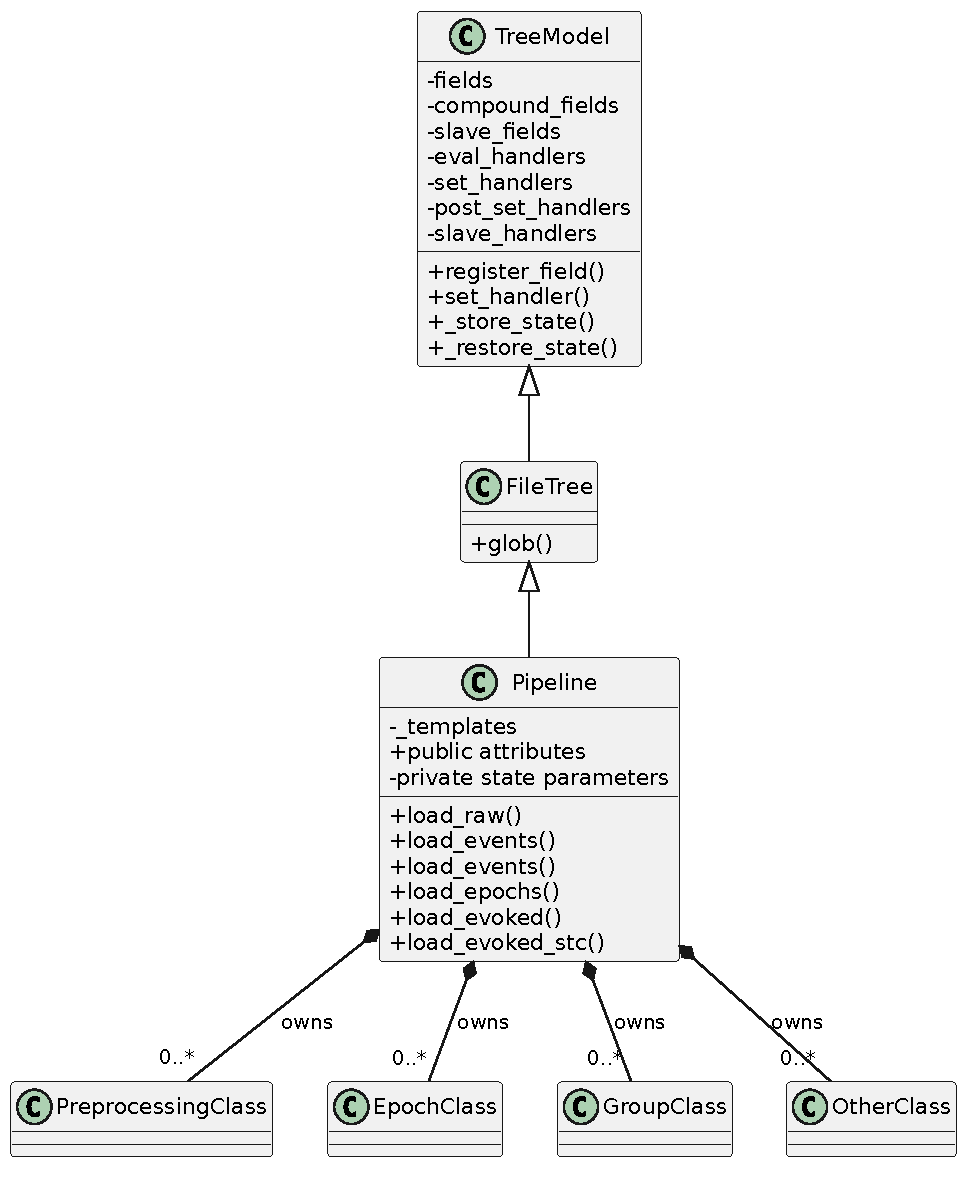
\includegraphics[width=0.65\textwidth]{../Resources/pipeline_design.pdf}

\end{frame}

%%%%%%%%%%%%%%%%%%%%%%%%%%%%%%%%%%%%%%

\begin{frame}

\frametitle{Abstraction to Isolate Interface}

\begin{itemize}

\item Eelbrain-BIDS
\begin{itemize}
  \item Changes mostly to Pipeline
  \item Missed path templating
\end{itemize}
\item Degree of abstraction depends on likelihood of change
\item Wrapper (Adapter) design pattern in trivial cases
\item Add strategy pattern for backward compatibility
\item Requires a mapping between the old and new interface
\item Not an option for Eelbrain-BIDS %since BIDS makes different assumptions about the data

\end{itemize}

\end{frame}

%%%%%%%%%%%%%%%%%%%%%%%%%%%%%%%%%%%%%%

\subsection[Implement]{Implementation}

%%%%%%%%%%%%%%%%%%%%%%%%%%%%%%%%%%%%%%

\begin{frame}

\frametitle{Implementation}

\begin{itemize}

\item Which library?
\begin{itemize}
  \item Performance, robustness, documentation quality, learning curve, community support, etc.
  \item Flexibility vs. simplicity
  \item Community size
\end{itemize}
\item \textbf{Task decomposition (helps non-experts)}
\item Assessing change impact, search code
\item Code reading using debug mode
\item Incremental iterative development
\item Eelbrain-BIDS
\begin{itemize}
  \item Upgrade parent classes first
  \item Domain knowledge in steps: preprocessing, epochs, source localization, etc.
  \item Stick with \texttt{mne.read\_raw\_fiff} over \texttt{mne-bids}
\end{itemize}

% For example, when we were considering using
% mne-bids to handle BIDS paths, we found that the documentation of read_raw_bids
% mentioned:
% “Will attempt to read associated events.tsv and channels.tsv files to populate the
% returned raw object with raw.annotations and raw.info['bads'].”
% This design is to save end user the effort of manually reading sidecar files (events.tsv
% and channels.tsv files). However, in Eelbrain, we already have good implementation
% of handling events and bad channels, so using this function blindly may cause unex-
% pected behaviour. Moreover, although using read_raw_bids to replace our logic looks
% convenient, we still want the flexibility of customizing this process in the future. There-
% fore, we decided to stick with mne.read_raw_fiff, though mne-bids looks “designed for
% BIDS”.

\end{itemize}

\end{frame}

%%%%%%%%%%%%%%%%%%%%%%%%%%%%%%%%%%%%%%

\subsection[Verification]{Verification}

%%%%%%%%%%%%%%%%%%%%%%%%%%%%%%%%%%%%%%

\begin{frame}

\frametitle{Verification and Documentation}

\begin{itemize}

\item Multi-layered testing (unit, integ., system)
\item Unit tests, integration tests, system tests
\item Reuse existing tests
\item Continuous integration (CI)
\item \textbf{Update documentation with each pull request} %chance for expert to review

\end{itemize}

\end{frame}

%%%%%%%%%%%%%%%%%%%%%%%%%%%%%%%%%%%%%%

\subsection[Migration]{Migration Plan}

%%%%%%%%%%%%%%%%%%%%%%%%%%%%%%%%%%%%%%

\begin{frame}

\frametitle{Migration Plan}

\begin{itemize}

\item Version number as clearest signal of breaking changes\footnote{\citet{preston-werner}}
\item Release notes
\item Deprecation warnings
\item Evolution models
\begin{itemize}
  \item Old and new interfaces coexist for a while, then old interface is deprecated
  \item Old interface is deprecated immediately (two in production)\footnote{\citet{LubkeEtAl2019}}
\end{itemize}
\item Eelbrain-BIDS uses two in production
\end{itemize}

% Release notes. This is the place to write comprehensive descriptions of the
% changes. In the release notes of the new version, we should clearly list all
% breaking changes, the reasons for them, and provide instructions on how to
% migrate existing scripts, if applicable. In Eelbrain, we listed the breaking changes
% in the version history section of the documentation.

% Deprecation warnings. This is the method trying to notify more users. In
% several versions before the breaking change, we can add deprecation warnings
% in the code, so that for a considerable time slot, when users run their existing
% scripts, they will see warnings about upcoming breaking changes. For Python
% packages, this can be done using the warnings module.

\end{frame}

%%%%%%%%%%%%%%%%%%%%%%%%%%%%%%%%%%%%%%

\section[Guidelines]{Guidelines}

%%%%%%%%%%%%%%%%%%%%%%%%%%%%%%%%%%%%%%

\section[Concluding Remarks]{Concluding Remarks}

\begin{frame}

\frametitle{Concluding Remarks}

\begin{itemize}

\item Case study: Eelbrain-BIDS
\item Steps
\begin{enumerate}
\item Should you standardize?
\item Backward compatibility?
\item Learn necessary domain knowledge
\item Document current design architecture
\item Abstraction to isolate interface
\item Implementation
\item Verification
\item Migration plan
\end{enumerate}
\item Guidelines/techniques
\begin{itemize}
  \item Question-driven learning
  \item Information hiding  
  \item Task decomposition
  \item Multi-layered testing 
  \item Deprecation warnings
\end{itemize}

\end{itemize}

\end{frame}

%%%%%%%%%%%%%%%%%%%%%%%%%%%%%%%%%%%%%%

\begin{frame}[allowframebreaks]
\frametitle{References}
\bibliography{../Resources/RSE-SSSS,../Resources/references} 
\bibliographystyle{plainnat}
\end{frame}

%%%%%%%%%%%%%%%%%%%%%%%%%%%%%%%%%%%%%%

\end{document}